\documentclass[a4paper, 11pt]{article}%
\usepackage[T1]{fontenc}%
\usepackage[utf8]{inputenc}%
\usepackage{lmodern}%
\usepackage{textcomp}%
\usepackage{lastpage}%
\usepackage{graphicx}%
%
\newcommand\tab[1][1cm]{\hspace*{#1}}%
\usepackage{fullpage}%
\usepackage{graphicx}%
%
\begin{document}%
\normalsize%
\noindent%
\large\textbf{Diamond Light Source Ltd} \hfill\large\textbf{Date: \today}%
\\\normalsize Beam Diagnostics Group \hfill\\%
\\\\
\includegraphics[width = 1\textwidth]{./Latex_Report/Logo.PNG}\\\\%
\section*{BPM Test Report}%
This is a \LaTeX test report for the, beam profile monitor electronics that are used at Diamond. In this document the different tests will be recorded in their own individual section. along with the specific parameters that are being tested and the test method used.\\\\%
\clearpage%
\tableofcontents%
\listoffigures%
\clearpage%
\section{Beam position equidistant grid raster scan test}%
Moves the beam position to -5 to 5 in the XY plane and recods beam position.
    The calc\_x\_pos and calc\_y\_pos functions are used to measure the theoretical beam position values.
    A set of ABCD values are created that will move the beam position from -5 to 5 in both the X and Y
    plane. This is then converted into attenuation values to put into the attenuator. A fixed RF frequency 
    and power is used while the attenuator values are changed. Finally the predicted values are compared 
    with the measured values of position. \\~\\
    Args:\\
        RFObject (RFSignalGenerator Obj): Object to interface with the RF hardware.\\
        BPMObject (BPMDevice Obj): Object to interface with the BPM hardware.\\
        ProgAttenObject (Prog\_Atten Obj): Object to interface with programmable attenuator hardware\\
        rf\_power (float): Output power of the RF system throughout the test, in dBm \\
        rf\_frequency (float): Frequency output of the RF throughout the test, in MHz\\
        nominal\_attenuation (float): starting attenuation values of each attenuator, in dB\\
        x\_points (int): number of samples in the X plane\\
        y\_points (int) number of samples in the Y plane \\
        settling\_time (float): time in seconds to wait between changing an attenuator value and 
            taking a reading from the BPM. \\
        ReportObject (LaTeX Report Obj): Specific report that the test results will be recorded 
            to. If no report is sent to the test then it will just display the results in 
            a graph. \\
        sub\_directory (str): String that can change where the graphs will be saved to\\~\\
    Returns:\\
        float array: measured X values of position\\
        float array: measured Y values of position\\
        float array: predicted X values of position\\
        float array: predicted Y values of position\\~\\
    %
\textbf{The devices used for this test are:}\\\\%
RF Source Rigol Technologies,DSG3030,DSG3B174500308,00.01.06\\%
Libera BPM with the Epics ID "libera:signals:fa" and the MAC Address "00:26:32:46:30:00"\\%
Programmable Attenuator RC4DAT-6G-95\\%
\\%
\textbf{The parameters used in this test are:}\\\\%
Fixed RF Output Power: -40dBm\\%
Fixed Rf Output Frequency: 499.6817682MHz\\%
Nominal Attenuation: 10dB\\%
Number of X points: 3\\%
Nunber of Y points: 3\\%
Settling time: 2s\\

%


\begin{figure}[htbp]%
\centering%
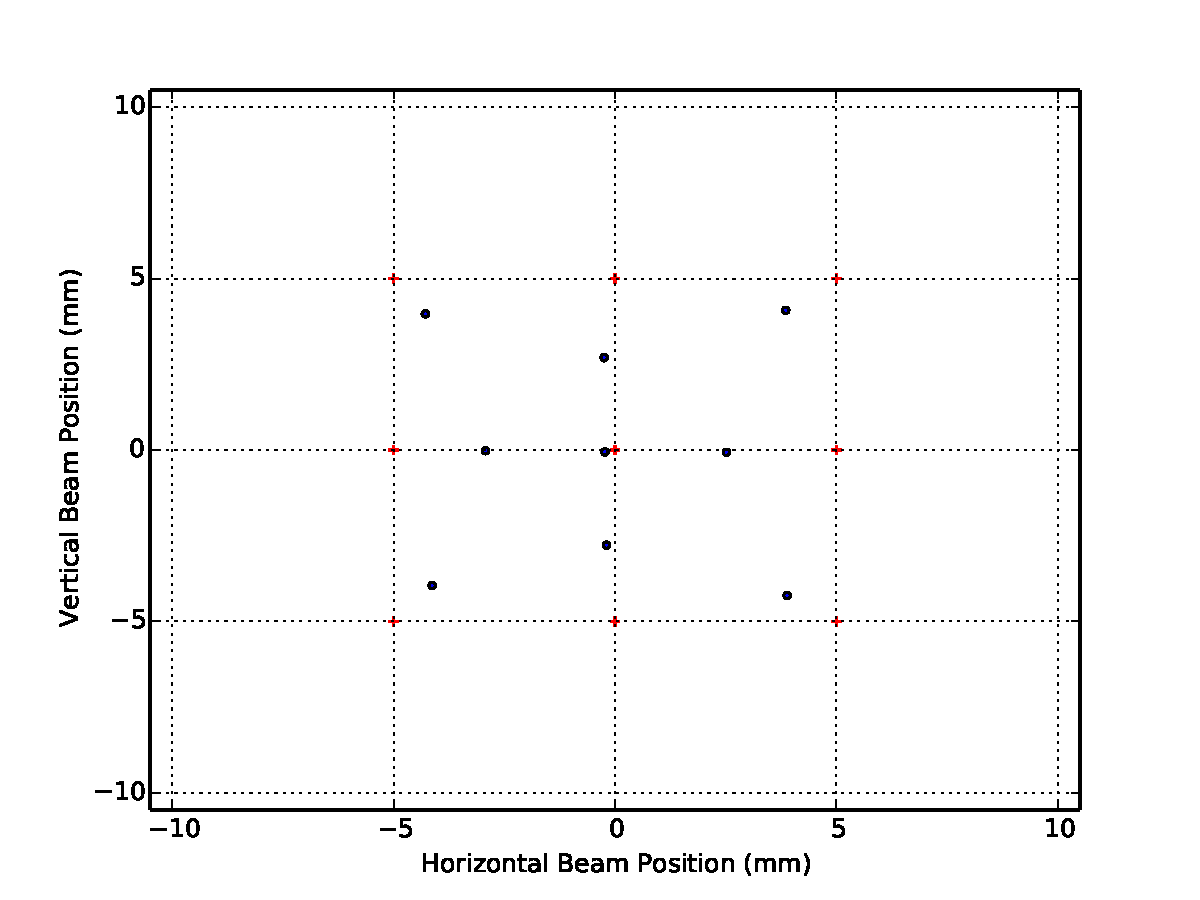
\includegraphics[width=0.8\textwidth]{./Results/Beam_position_equidistant_grid_raster_scan_test}%
\caption{}%
\end{figure}

%
\clearpage%
\section{beam\_position\_attenuation\_permutation}%
"Moves the beam position by changing the attenuator values with a series of different permutations.
    The calc\_x\_pos and calc\_y\_pos functions are used to measure the theoretical beam position values.
    The attenuator\_max, attenuator\_min and attenuator\_steps are used to create a series of different 
    combinations of attenuator values. A linear space will be made from the min to the max value of 
    attenuation. These values will then be put into all possible permutations with four values. Each 
    permutation will be fed to the four attenuators, and the BPM position recoded after each 
    attenuation change. \\~\\
    Args:\\
        RFObject (RFSignalGenerator Obj): Object to interface with the RF hardware.\\
        BPMObject (BPMDevice Obj): Object to interface with the BPM hardware.\\
        ProgAttenObject (Prog\_Atten Obj): Object to interface with programmable attenuator hardware\\
        rf\_power (float): Output power of the RF system throughout the test, in dBm \\
        rf\_frequency (float): Frequency output of the RF throughout the test, in MHz\\
        attenuator\_max (float): max value for the attenuators\\
        attenuator\_min (float): min value for the attenuators\\
        attenuator\_steps (float): steps between the min and max values\\
        settling\_time (float): time in seconds to wait between changing an attenuator value and 
            taking a reading from the BPM. \\
        ReportObject (LaTeX Report Obj): Specific report that the test results will be recorded 
            to. If no report is sent to the test then it will just display the results in 
            a graph. \\
        sub\_directory (str): String that can change where the graphs will be saved to\\~\\
    Returns:\\
        float array: measured X values of position\\
        float array: measured Y values of position\\
        float array: predicted X values of position\\
        float array: predicted Y values of position\\~\\
    %
\textbf{The devices used for this test are:}\\\\%
RF Source Rigol Technologies,DSG3030,DSG3B174500308,00.01.06\\%
Libera BPM with the Epics ID "libera:signals:fa" and the MAC Address "00:26:32:46:30:00"\\%
Programmable Attenuator RC4DAT-6G-95\\%
\\%
\textbf{The parameters used in this test are:}\\\\%
Fixed RF Output Power: -40 dBm\\%
Fixed Rf Output Frequency: 499.6817682 MHz\\%
Maximum Attenuation: 50dB\\%
Minimum Attenuation: 10dB\\%
Steps between min and max attenuations: 2\\%
Settling time: 2s\\

%


\begin{figure}[htbp]%
\centering%
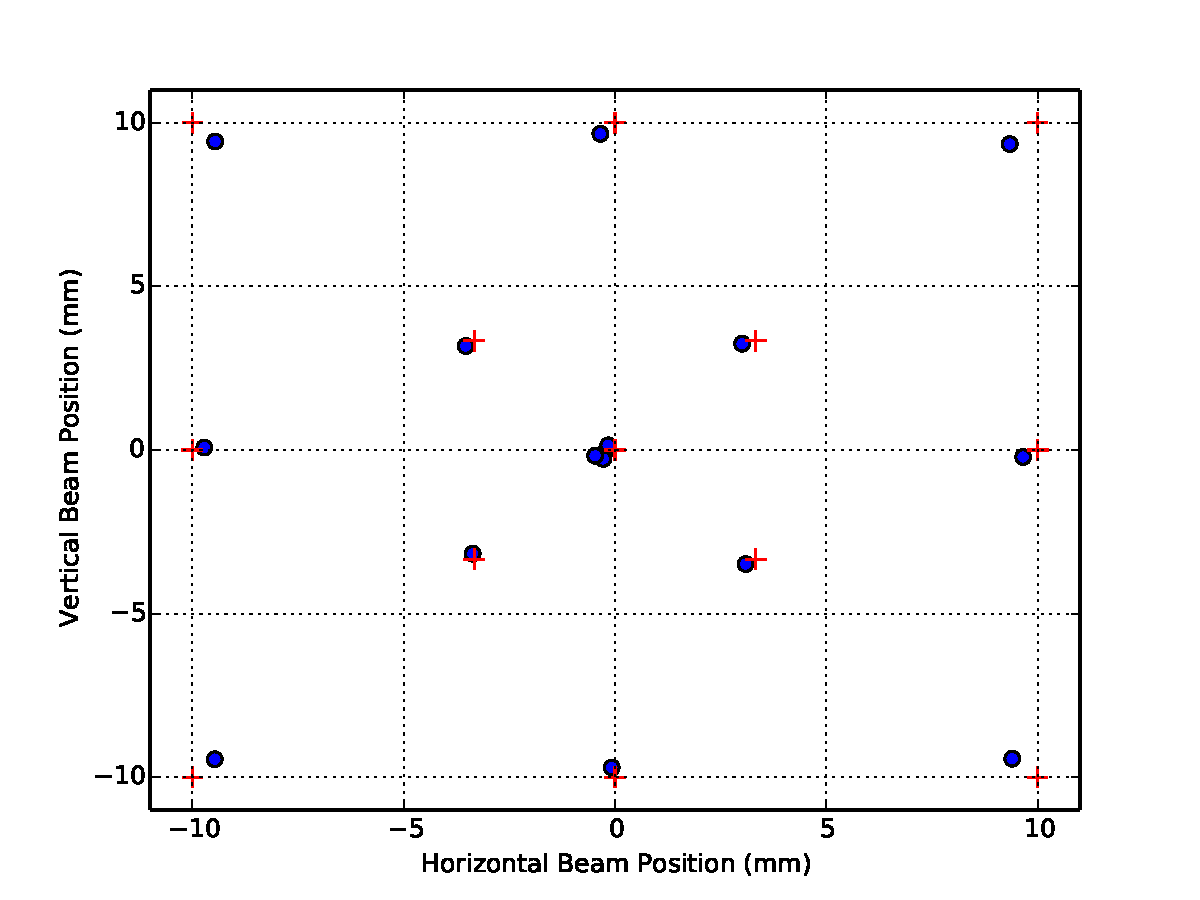
\includegraphics[width=0.8\textwidth]{./Results/beam_position_attenuation_permutation}%
\caption{}%
\end{figure}

%
\clearpage%
\section{Beam Power Dependance}%
Tests the relationship between RF output power and values read from the BPM. 
    An RF signal is output, and then different parameters are measured from the BPM. 
    The signal is linearly ramped up in dBm at a single frequency. The number of samples to take, 
    and settling time between each measurement can be decided using the arguments. \\~\\
    Args:\\
        RFObject (RFSignalGenerator Obj): Object to interface with the RF hardware.\\
        BPMObject (BPMDevice Obj): Object to interface with the BPM hardware.\\
        frequency (float): Output frequency for the tests, set as a float that will 
            use the assumed units of MHz. \\
        start\_power (float): Starting output power for the tests, default value is 
            -100 dBm. The input values are floats and dBm is assumed. \\
        end\_power (float): Final output power for the tests, default value is 0 dBm.
            The input values are floats and dBm assumed. \\
        samples (int): Number of samples take is this value + 1.\\
        settling\_time (float): Time in seconds, that the program will wait in between 
            setting an  output power on the RF, and reading the values of the BPM. \\
        ReportObject (LaTeX Report Obj): Specific report that the test results will be recorded 
            to. If no report is sent to the test then it will just display the results in 
            a graph. \\
        sub\_directory (str): String that can change where the graphs will be saved to.\\~\\
    Returns:\\
        float array: Power output from the RF\\
        float array: Power read at the BPM\\
        float array: Beam Current read at the BPM\\
        float array: X Positions read from the BPM\\
        float array: Y Positions read from the BPM\\~\\
    %
\textbf{The devices used for this test are:}\\\\%
RF Source Rigol Technologies,DSG3030,DSG3B174500308,00.01.06\\%
Libera BPM with the Epics ID "libera:signals:fa" and the MAC Address "00:26:32:46:30:00"\\%
\\%
\textbf{The parameters used in this test are:}\\\\%
Frequency: 499.6817682MHz\\%
Starting output power: -100dBm\\%
Final output power: -40dBm\\%
Samples: 10\\%
Settling time: 2s\\

%
\begin{figure}[htbp]%
\centering%
\caption{Beam Power Dependence Results}%
\begin{tabular}{|c|c|c|c|c|c|}%
\hline%
Output Power&Input Power&BPM Current&X Position&Y Position&ADC Sum\\%
(dBm)&(dBm)&(mA)&(mm)&(mm)&(Counts)\\%
\hline%
{-}100.0&7601.09&7601.09&{-}0.49&{-}0.2&7601.0\\%
{-}93.33&8194.41&8194.41&{-}0.5&{-}0.22&8194.0\\%
{-}86.67&10663.84&10663.84&{-}0.51&{-}0.2&10664.0\\%
{-}80.0&19509.3&19509.3&{-}0.41&{-}0.1&19509.0\\%
{-}73.33&42573.4&42573.4&{-}0.27&{-}0.04&42573.0\\%
{-}66.67&90774.86&90774.86&{-}0.25&{-}0.03&90775.0\\%
{-}60.0&198232.72&198232.72&{-}0.23&{-}0.03&198233.0\\%
{-}53.33&426933.58&426933.58&{-}0.22&{-}0.03&426934.0\\%
{-}46.67&909240.3&909240.3&{-}0.21&{-}0.03&909240.0\\%
{-}40.0&1960738.74&1960738.74&{-}0.19&{-}0.0&1960739.0\\%
\hline%
\end{tabular}%
\end{figure}%


\begin{figure}[htbp]%
\centering%
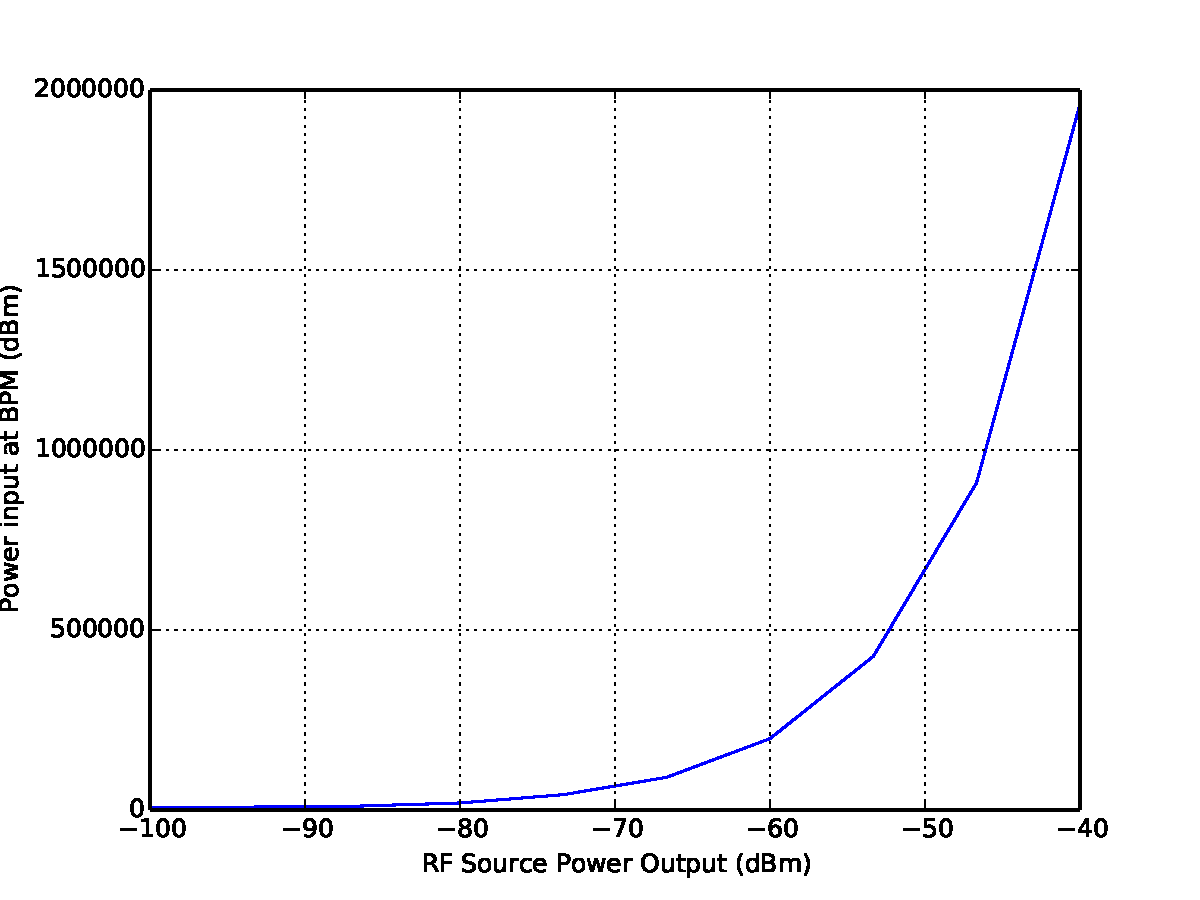
\includegraphics[width=0.8\textwidth]{./Results/power_vs_power.pdf}%
\caption{}%
\end{figure}

%


\begin{figure}[htbp]%
\centering%
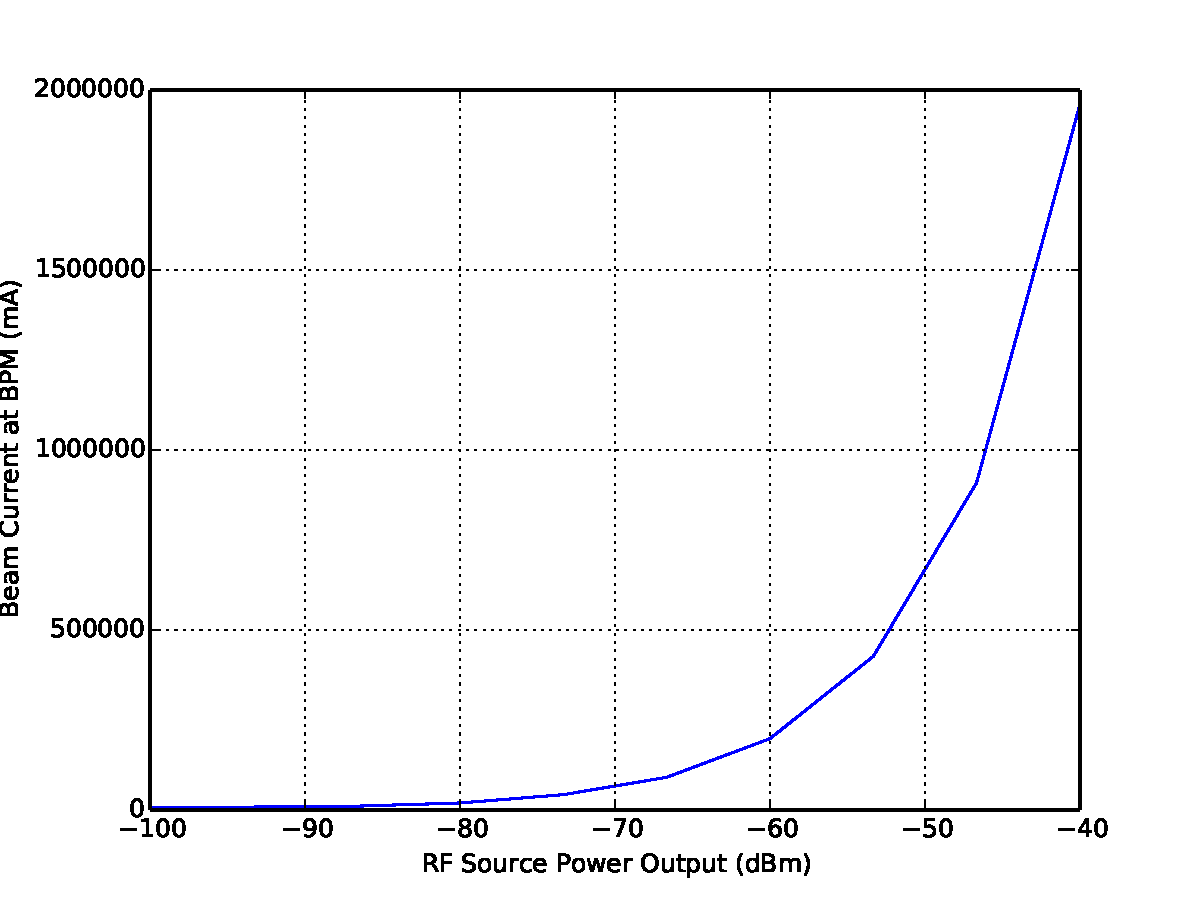
\includegraphics[width=0.8\textwidth]{./Results/power_vs_current.pdf}%
\caption{}%
\end{figure}

%


\begin{figure}[htbp]%
\centering%
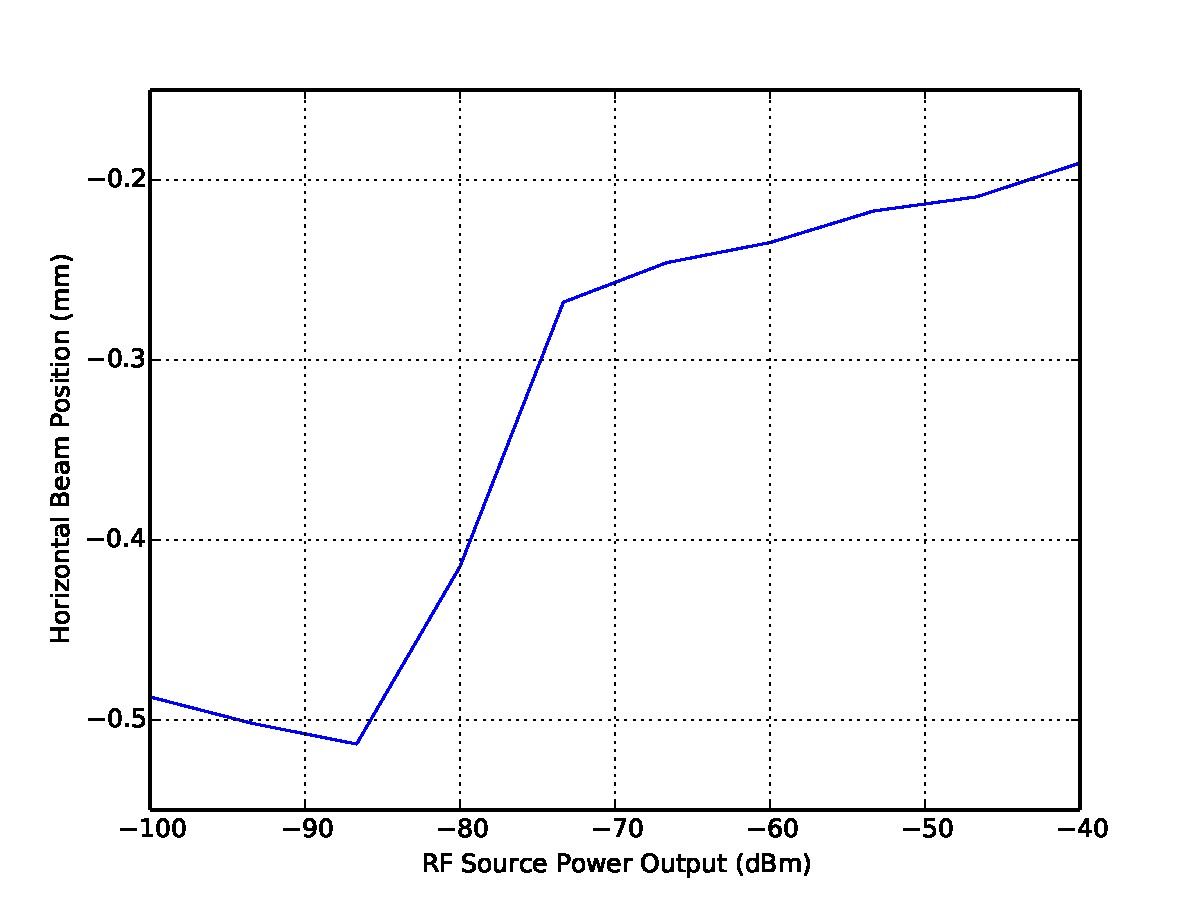
\includegraphics[width=0.8\textwidth]{./Results/power_vs_X.pdf}%
\caption{}%
\end{figure}

%


\begin{figure}[htbp]%
\centering%
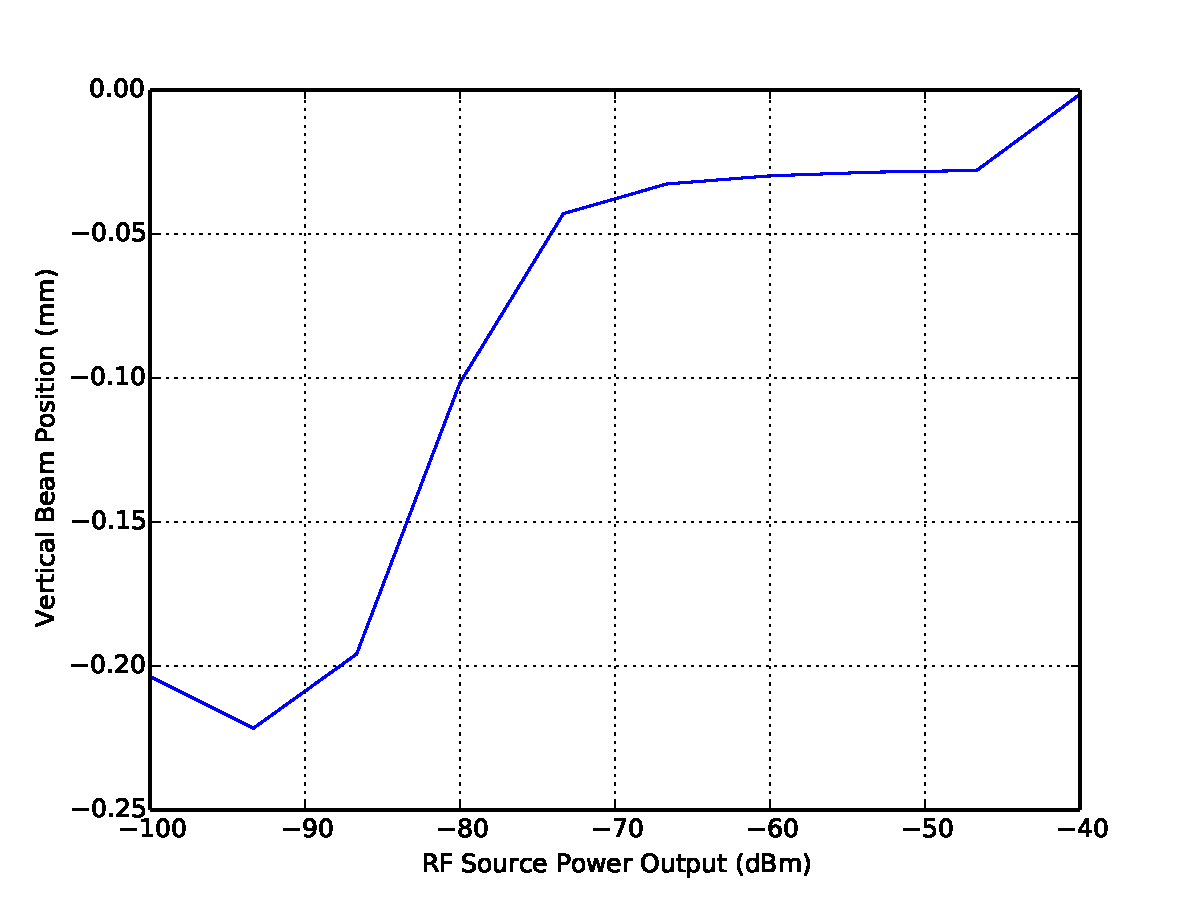
\includegraphics[width=0.8\textwidth]{./Results/power_vs_Y.pdf}%
\caption{}%
\end{figure}

%


\begin{figure}[htbp]%
\centering%
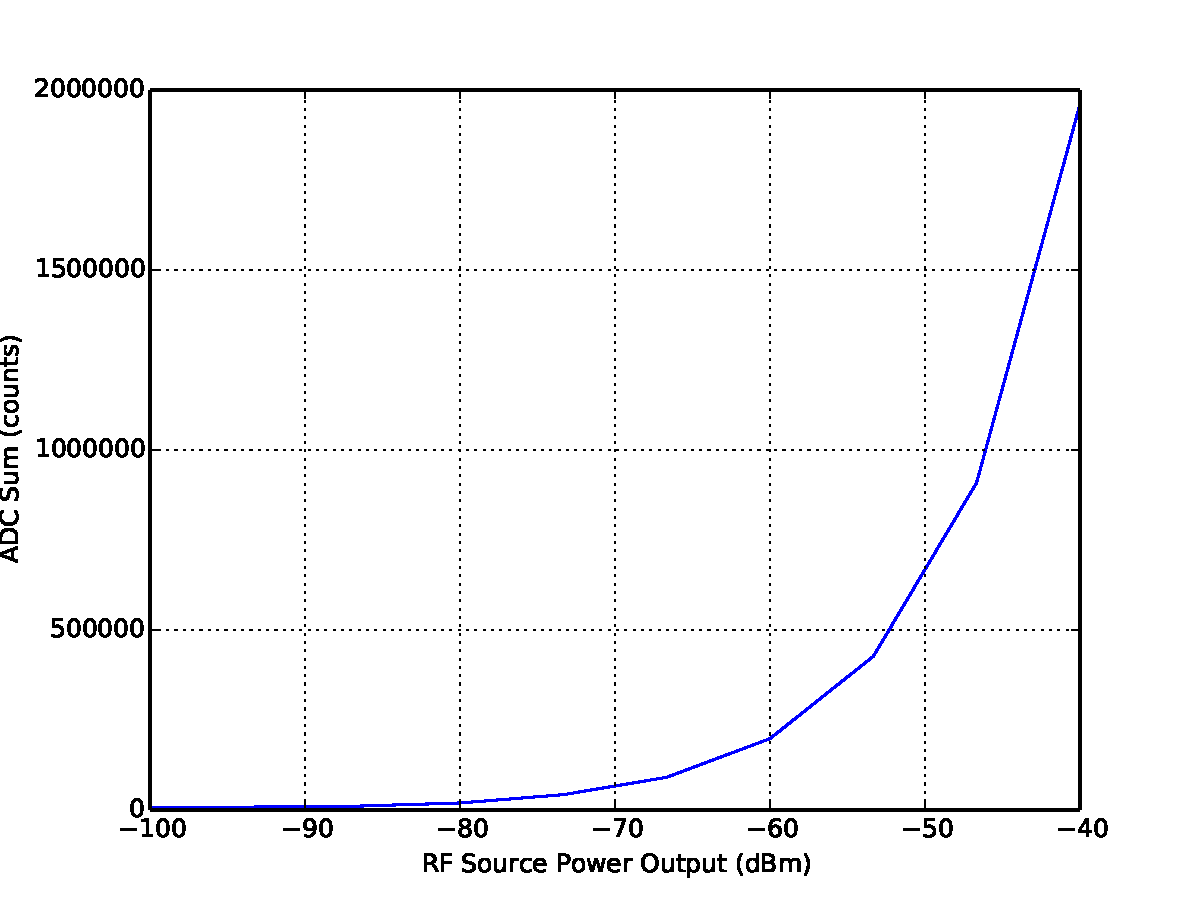
\includegraphics[width=0.8\textwidth]{./Results/power_vs_ADC_sum.pdf}%
\caption{}%
\end{figure}

%
\clearpage%
\section{Fixed voltage amplitude fill pattern test}%

        This test imitates a fill pattern by modulation the RF signal with a square wave. The up time 
        of the square wave represents when a bunch goes passed, and the downtime the gaps between the 
        bunches. This test will take the pulse length in micro seconds, and then linearly step up the 
        duty cycle of the pulse, from 0.1 to 1. Readings on the BPM are then recorded as the duty cycle
        is changed. While the duty cycle is increased, the peak RF voltage stays fixed, meaning that 
        the average power will change with duty cycle. \\~\\
        Args:\\
            RFObject (RFSignalGenerator Obj): Object to interface with the RF hardware.\\
            BPMObject (BPMDevice Obj): Object to interface with the BPM hardware.\\
            GateSourceObject: (GateSource Obj): Object used to interface with the gate source hardware. \\
            frequency (float/str): Output frequency for the tests, set as a float that will use the assumed units of MHz. \\
            power (float): Starting output power for the tests, default value is -100 dBm. The input values are floats and dBm is assumed. \\
            samples (int): Number of samples take is this value + 1.\\
            pulse\_period (float): The pulse period for the modulation signal, i.e. the bunch length, this is a float that is in micro seconds.\\
            settling\_time (float): Time in seconds, that the program will wait in between setting an  output power on the RF, and reading the values of the BPM. \\
            ReportObject (LaTeX Report Obj): Specific report that the test results will be recorded to. If no report is sent to the test then it will just display the results in a graph. \\
            sub\_directory (str): String that can change where the graphs will be saved to\\~\\  
        Returns:\\
            float array: duty cycle of the modulation signal\\
            float array: power read from the BPM\\
            float array: current read from the BPM\\
            float array: X position read from the BPM\\
            float array: Y position read from the BPM\\~\\  
    %
\textbf{The devices used for this test are:}\\\\%
RF Source Rigol Technologies,DSG3030,DSG3B174500308,00.01.06\\%
Gating Device Rigol Technologies,DSG3030,DSG3B174500308,00.01.06\\%
Libera BPM with the Epics ID "libera:signals:fa" and the MAC Address "00:26:32:46:30:00"\\%
\\%
\textbf{The parameters used in this test are:}\\\\%
Frequency: 499.681 768 20MHz\\%
Output Power: -40.00DBM\\%
Pulse Period: 1.873us\\%
Samples: 10\\%
Settling time: 2s\\

%
\begin{figure}[htbp]%
\centering%
\caption{Changing gate duty cycle, with fixed RF amplitude }%
\begin{tabular}{|c|c|c|c|c|c|}%
\hline%
Duty Cycle&Input Power&BPM Current&X Position&Y Position&ADC Sum\\%
(0{-}1)&(dBm)&(mA)&(mm)&(mm)&(Counts)\\%
\hline%
0.1&180545.97&180545.97&{-}0.2&{-}0.0&180546.0\\%
0.2&372144.17&372144.17&{-}0.2&{-}0.0&372144.0\\%
0.3&553962.57&553962.57&{-}0.19&{-}0.0&553963.0\\%
0.4&746432.06&746432.06&{-}0.19&{-}0.0&746432.0\\%
0.5&939421.27&939421.27&{-}0.19&{-}0.0&939421.0\\%
0.6&1133596.25&1133596.25&{-}0.19&{-}0.0&1133596.0\\%
0.7&1317615.57&1317615.57&{-}0.19&{-}0.0&1317616.0\\%
0.8&1513679.99&1513679.99&{-}0.19&{-}0.0&1513680.0\\%
0.9&1711722.35&1711722.35&{-}0.19&{-}0.0&1711722.0\\%
0.99&1923383.42&1923383.42&{-}0.19&{-}0.0&1923383.0\\%
\hline%
\end{tabular}%
\end{figure}%


\begin{figure}[htbp]%
\centering%
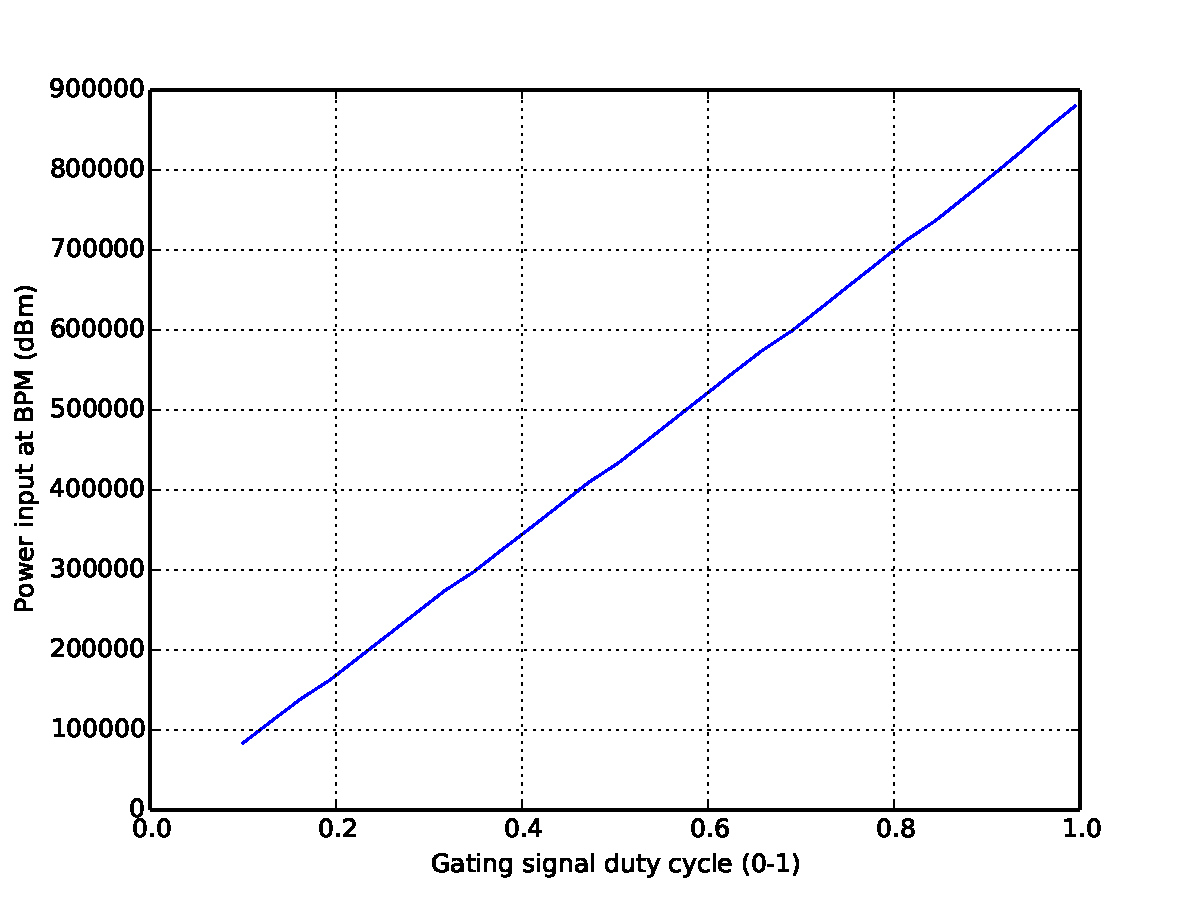
\includegraphics[width=0.8\textwidth]{./Results/DC_vs_power.pdf}%
\caption{}%
\end{figure}

%


\begin{figure}[htbp]%
\centering%
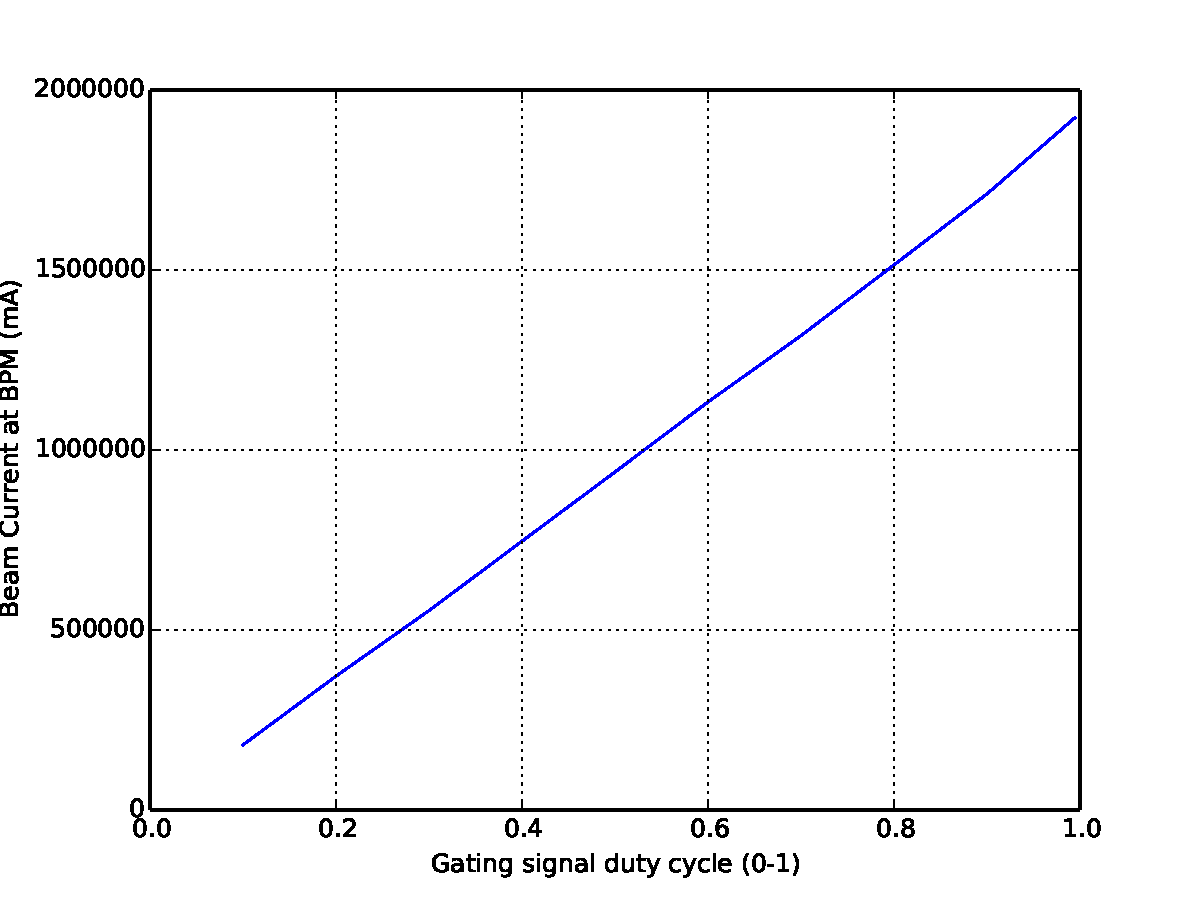
\includegraphics[width=0.8\textwidth]{./Results/DC_vs_current.pdf}%
\caption{}%
\end{figure}

%


\begin{figure}[htbp]%
\centering%
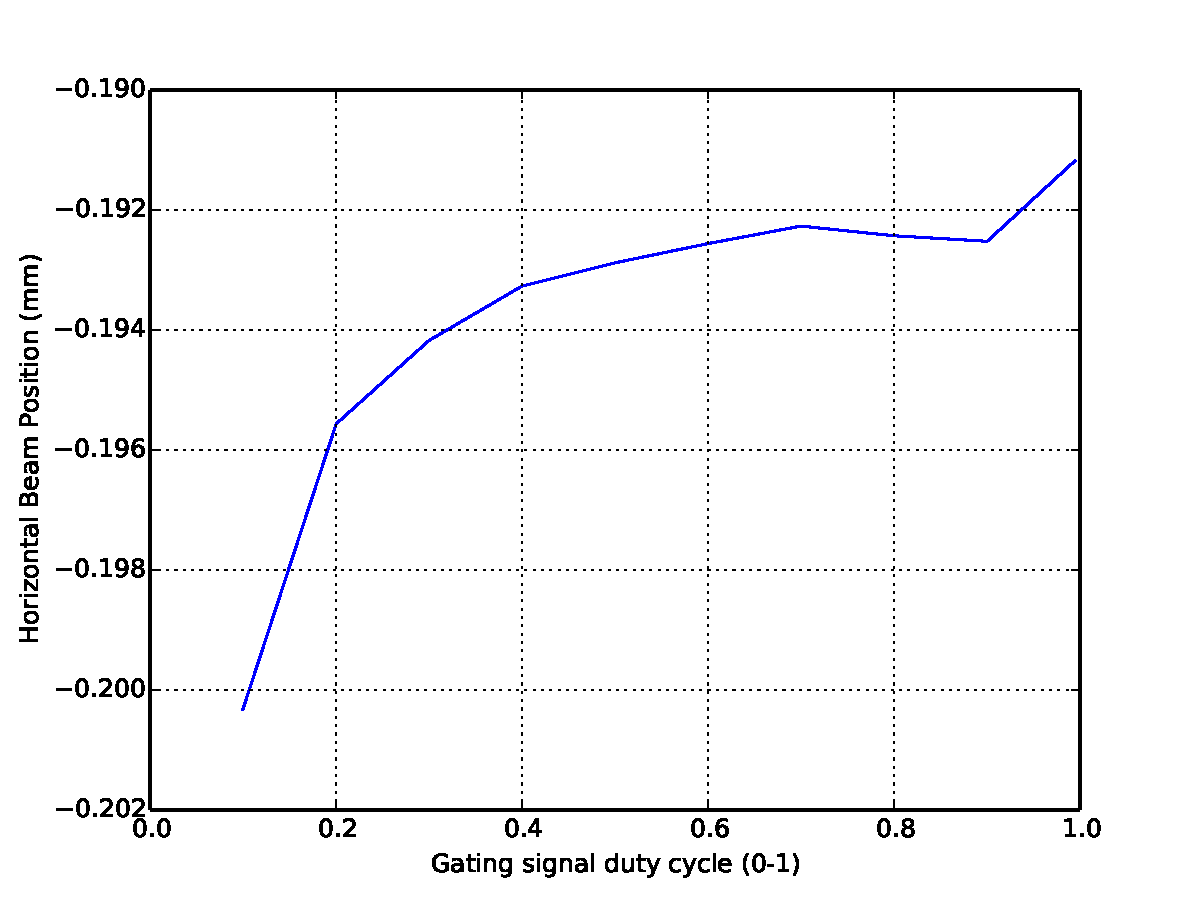
\includegraphics[width=0.8\textwidth]{./Results/DC_vs_X.pdf}%
\caption{}%
\end{figure}

%


\begin{figure}[htbp]%
\centering%
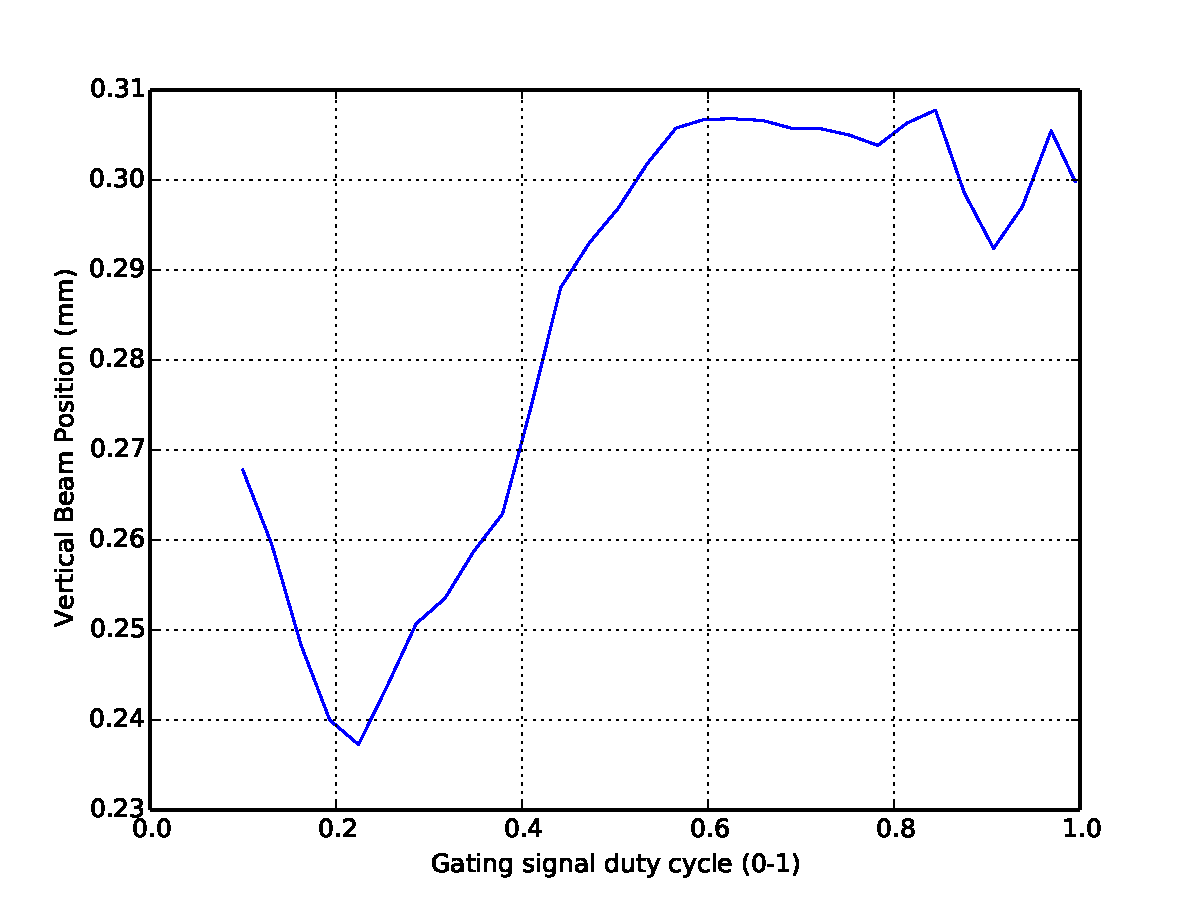
\includegraphics[width=0.8\textwidth]{./Results/DC_vs_Y.pdf}%
\caption{}%
\end{figure}

%


\begin{figure}[htbp]%
\centering%
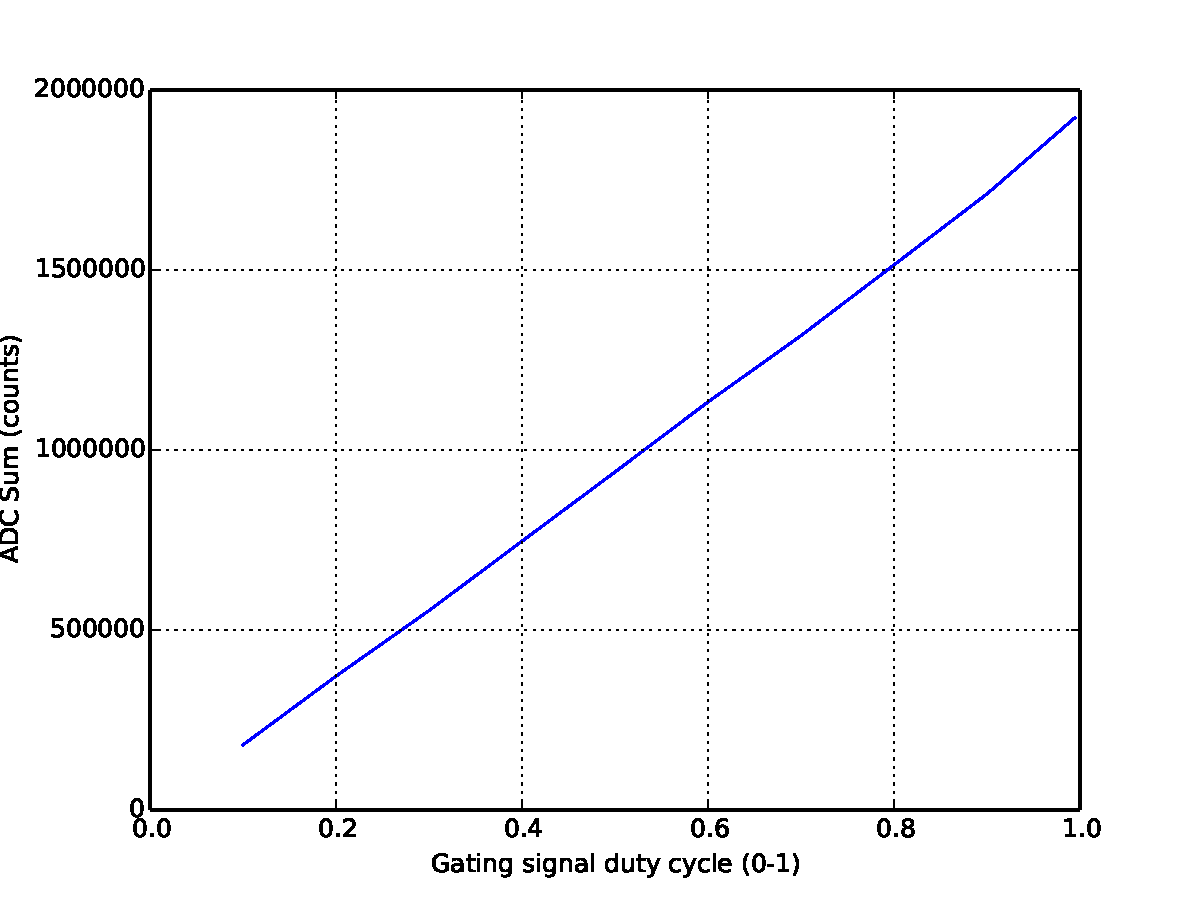
\includegraphics[width=0.8\textwidth]{./Results/DC_vs_ADC_sum.pdf}%
\caption{}%
\end{figure}

%
\clearpage%
\section{Scaled voltage amplitude fill pattern test}%

        This test imitates a fill pattern by modulation the RF signal with a square wave. The up time 
        of the square wave represents when a bunch goes passed, and the downtime the gaps between the 
        bunches. This test will take the pulse length in micro seconds, and then linearly step up the 
        duty cycle of the pulse, from 0.1 to 1. Readings on the BPM are then recorded as the duty cycle
        is changed. While the duty cycle is increased, the peak RF voltage increases, meaning that 
        the average power will be constant with duty cycle change. \\~\\
        Args:\\
            RFObject (RFSignalGenerator Obj): Object to interface with the RF hardware.\\
            BPMObject (BPMDevice Obj): Object to interface with the BPM hardware.\\
            GateSourceObject: (GateSource Obj): Object used to interface with the gate source hardware. \\
            frequency (float/str): Output frequency for the tests, set as a float that will use the assumed units of MHz. \\
            desired\_power (float): Starting output power for the tests, default value is -40 dBm. The input values are floats and dBm is assumed. \\
            samples (int): Number of samples take is this value + 1.\\
            pulse\_period (float): The pulse period for the modulation signal, i.e. the bunch length, this is a float that is in micro seconds. \\
            settling\_time (float): Time in seconds, that the program will wait in between setting an  output power on the RF, and reading the values of the BPM. \\
            ReportObject (LaTeX Report Obj): Specific report that the test results will be recorded to. If no report is sent to the test then it will just display the results in a graph. \\
            sub\_directory (str): String that can change where the graphs will be saved to \\~\\ 
        Returns:\\
            float array: duty cycle of the modulation signal \\
            float array: power set at the rf output \\
            float array: power read from the BPM \\
            float array: current read fro mthe BPM \\
            float array: X position read from the BPM \\
            float array: Y position read from the BPM \\~\\  
    %
\textbf{The devices used for this test are:}\\\\%
RF Source Rigol Technologies,DSG3030,DSG3B174500308,00.01.06\\%
Gating Device Rigol Technologies,DSG3030,DSG3B174500308,00.01.06\\%
Libera BPM with the Epics ID "libera:signals:fa" and the MAC Address "00:26:32:46:30:00"\\%
\\%
\textbf{The parameters used in this test are:}\\\\%
Frequency: 499.681 768 20MHz\\%
Desired Power: -70dBm\\%
Pulse Period: 1.873us\\%
Samples: 10\\%
Settling time: 2s\\

%
\begin{figure}[htbp]%
\centering%
\caption{Changing gate duty cycle, with fixed RF amplitude }%
\begin{tabular}{|c|c|c|c|c|c|c|}%
\hline%
Duty Cycle&Output Power&Input Power&BPM Current&X Position&Y Position&ADC Sum\\%
(0{-}1)&(dBm)&(dBm)&(mA)&(mm)&(mm)&(Counts)\\%
\hline%
0.1&{-}49.99&58003.9&58003.9&{-}0.23&{-}0.04&58004.0\\%
0.2&{-}56.03&55671.16&55671.16&{-}0.23&{-}0.03&55671.0\\%
0.3&{-}59.54&59570.92&59570.92&{-}0.25&{-}0.03&59571.0\\%
0.4&{-}62.04&59652.74&59652.74&{-}0.25&{-}0.03&59653.0\\%
0.5&{-}63.98&61292.11&61292.11&{-}0.24&{-}0.03&61292.0\\%
0.6&{-}65.56&60659.01&60659.01&{-}0.24&{-}0.04&60659.0\\%
0.7&{-}66.9&60460.97&60460.97&{-}0.24&{-}0.03&60461.0\\%
0.8&{-}68.06&60689.64&60689.64&{-}0.23&{-}0.03&60690.0\\%
0.9&{-}69.09&57347.08&57347.08&{-}0.24&{-}0.03&57347.0\\%
0.99&{-}69.95&57471.3&57471.3&{-}0.24&{-}0.04&57471.0\\%
\hline%
\end{tabular}%
\end{figure}%


\begin{figure}[htbp]%
\centering%
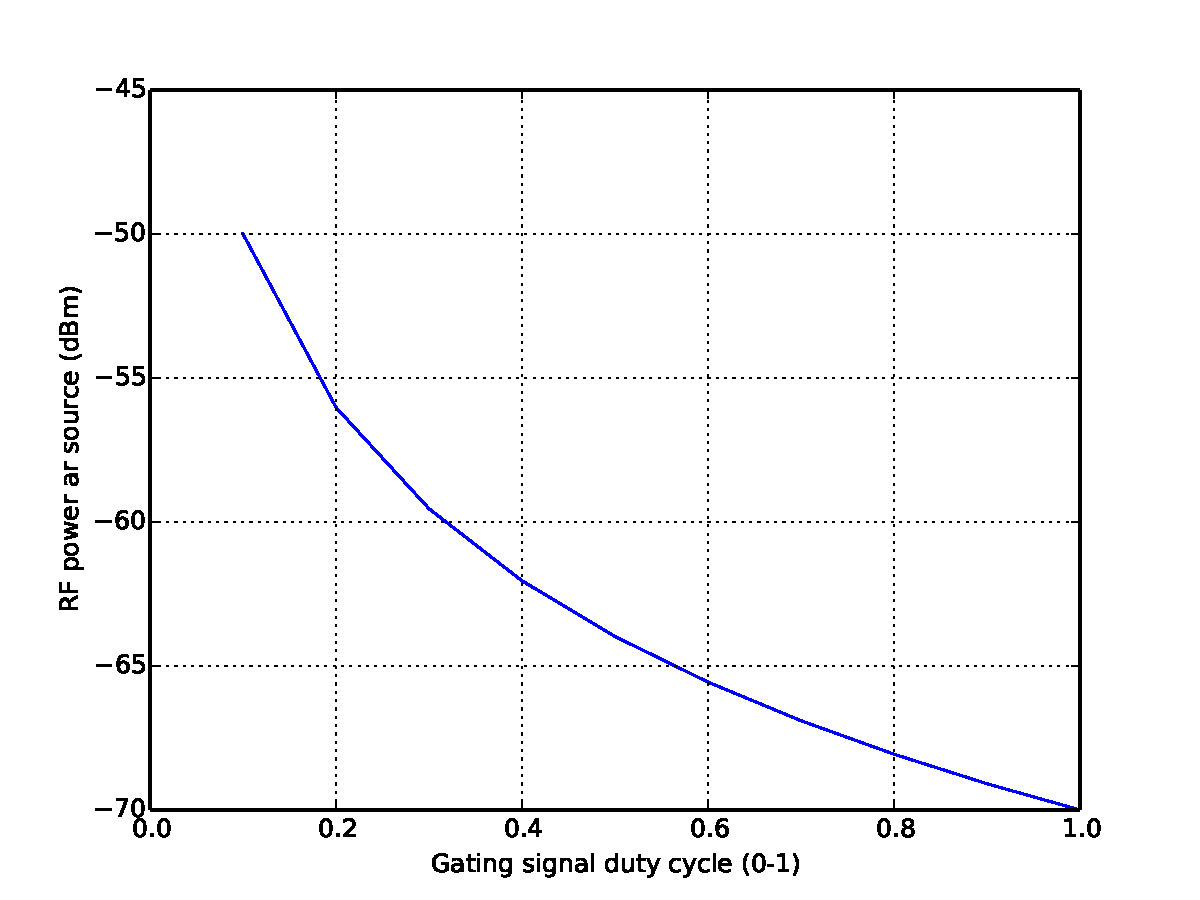
\includegraphics[width=0.8\textwidth]{./Results/scaled_DC_vs_Out_power.pdf}%
\caption{}%
\end{figure}

%


\begin{figure}[htbp]%
\centering%
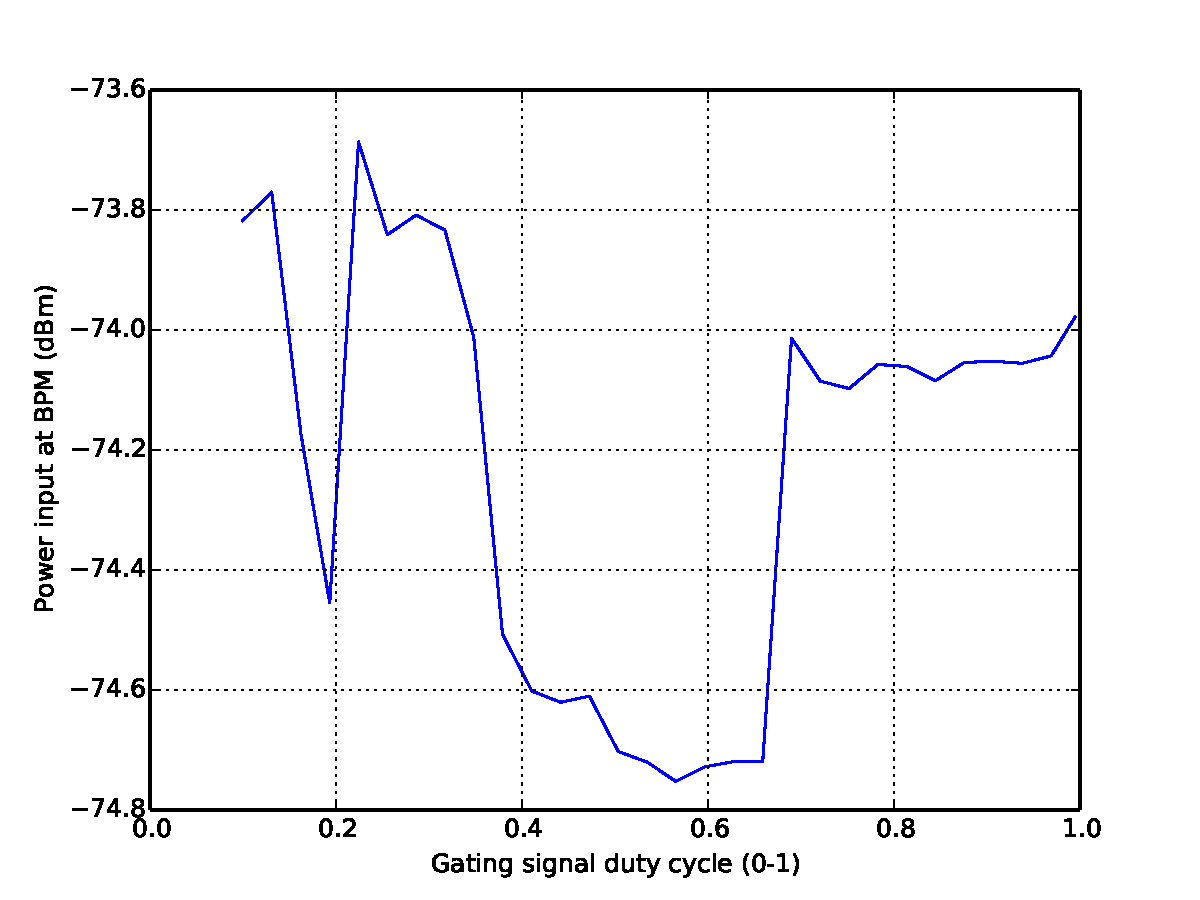
\includegraphics[width=0.8\textwidth]{./Results/scaled_DC_vs_In_power.pdf}%
\caption{}%
\end{figure}

%


\begin{figure}[htbp]%
\centering%
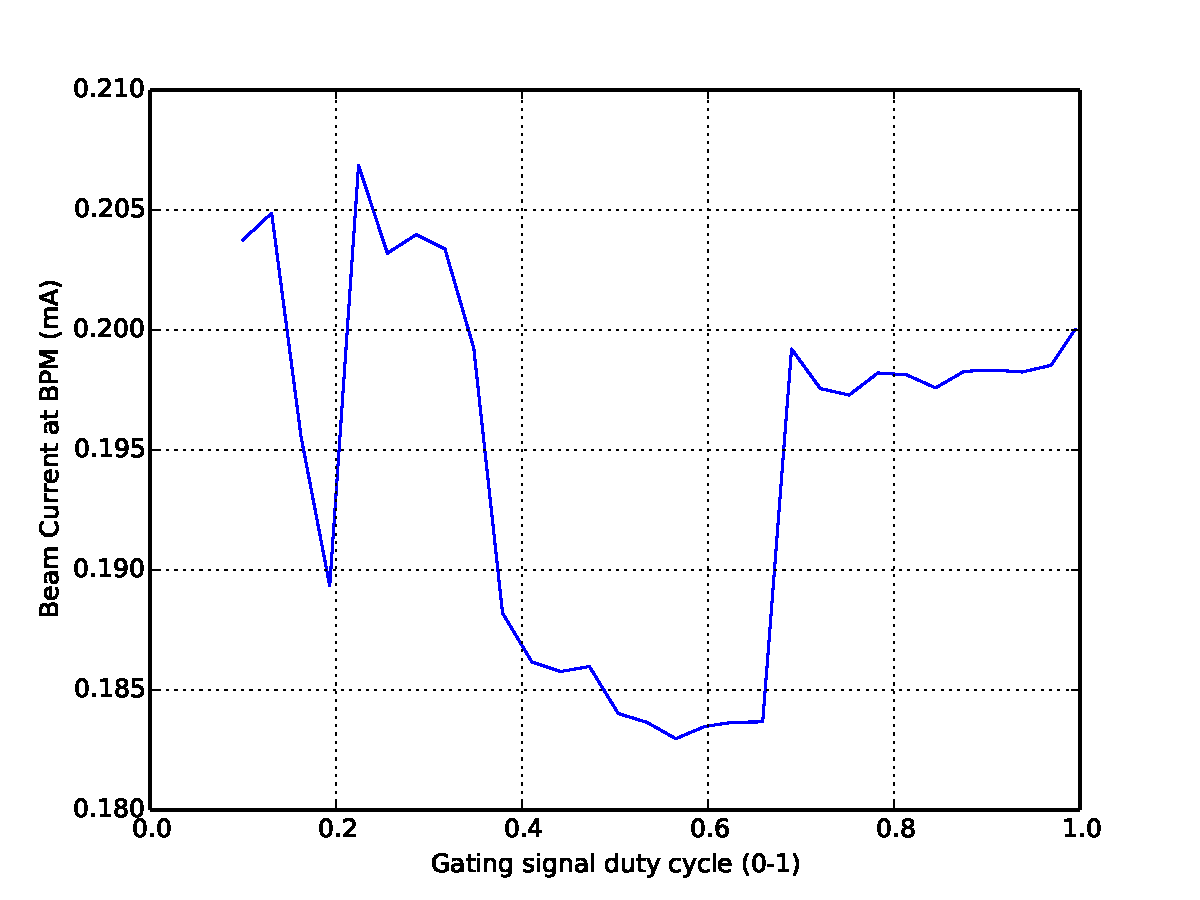
\includegraphics[width=0.8\textwidth]{./Results/scaled_DC_vs_current.pdf}%
\caption{}%
\end{figure}

%


\begin{figure}[htbp]%
\centering%
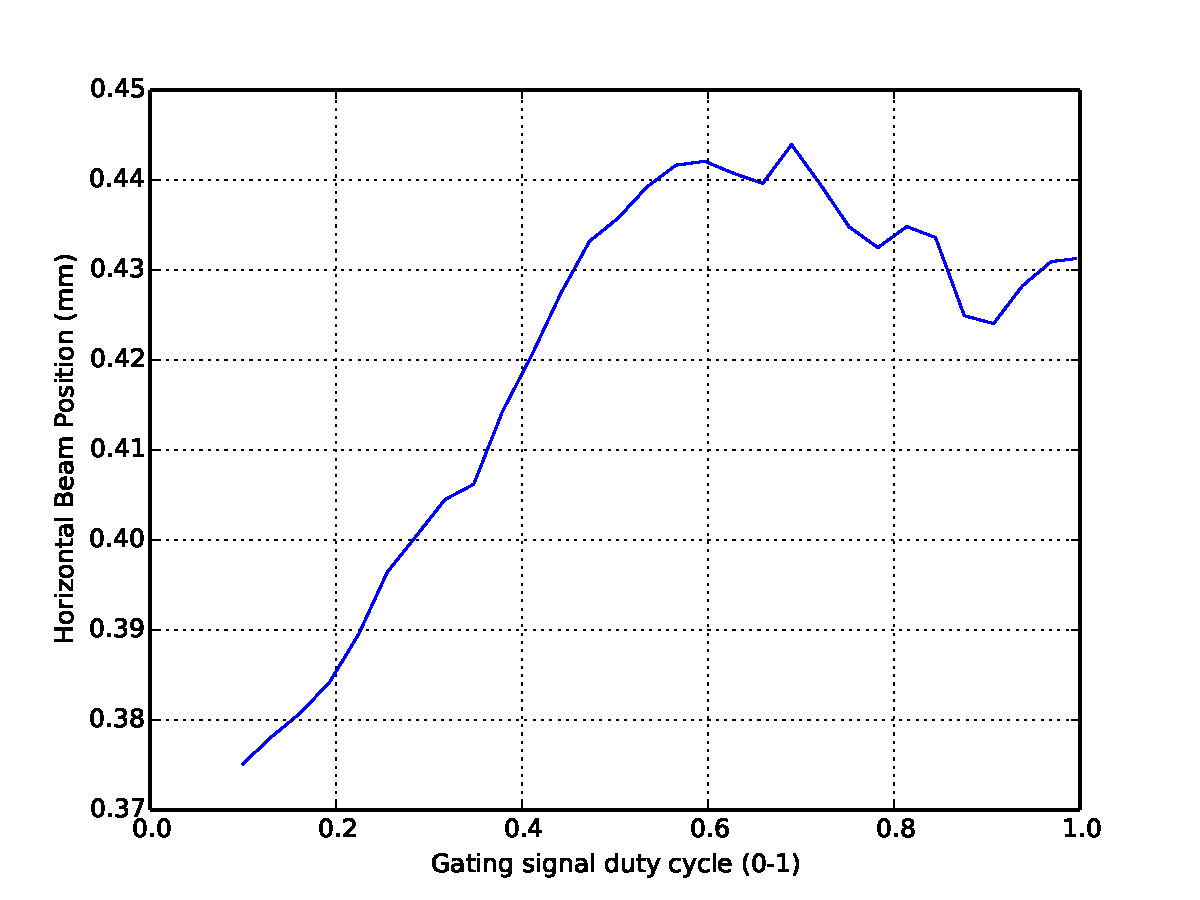
\includegraphics[width=0.8\textwidth]{./Results/scaled_DC_vs_X.pdf}%
\caption{}%
\end{figure}

%


\begin{figure}[htbp]%
\centering%
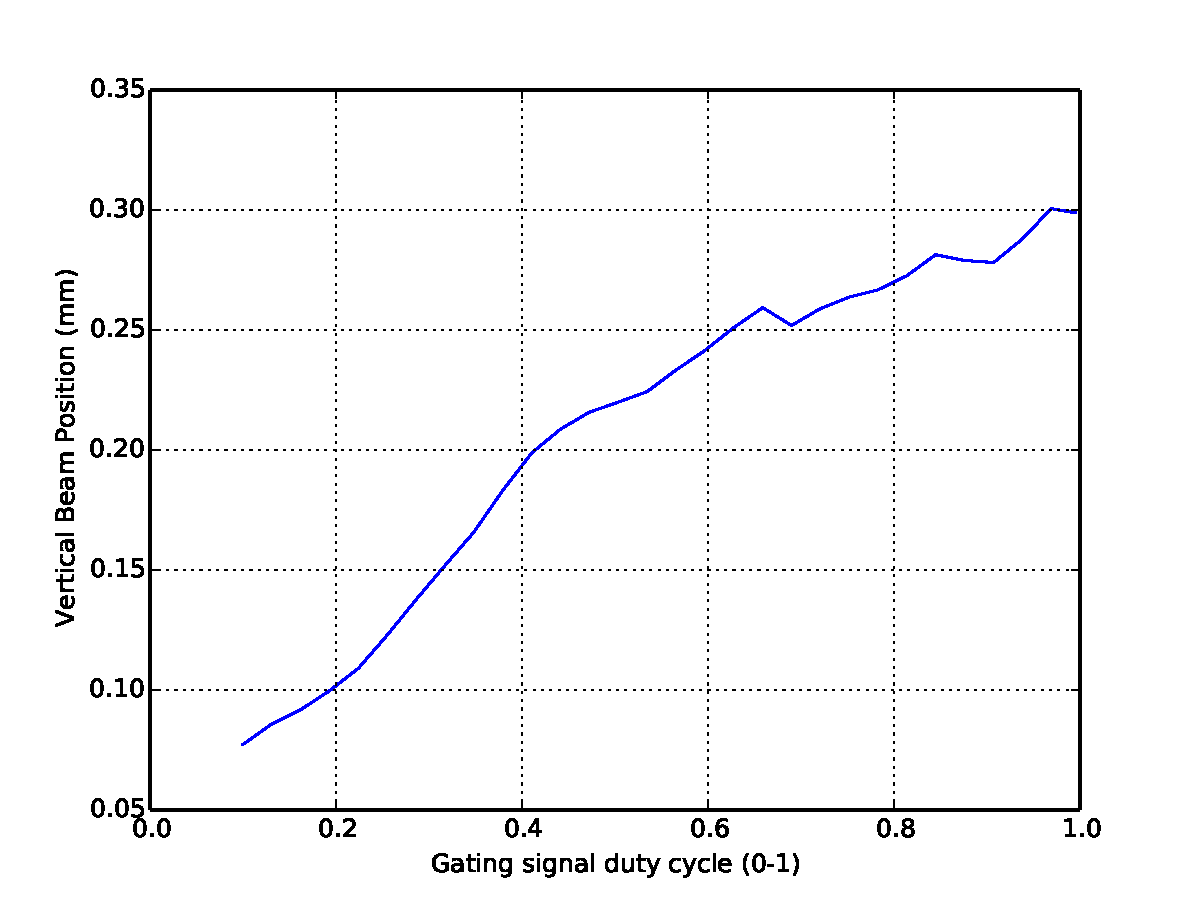
\includegraphics[width=0.8\textwidth]{./Results/scaled_DC_vs_Y.pdf}%
\caption{}%
\end{figure}

%


\begin{figure}[htbp]%
\centering%
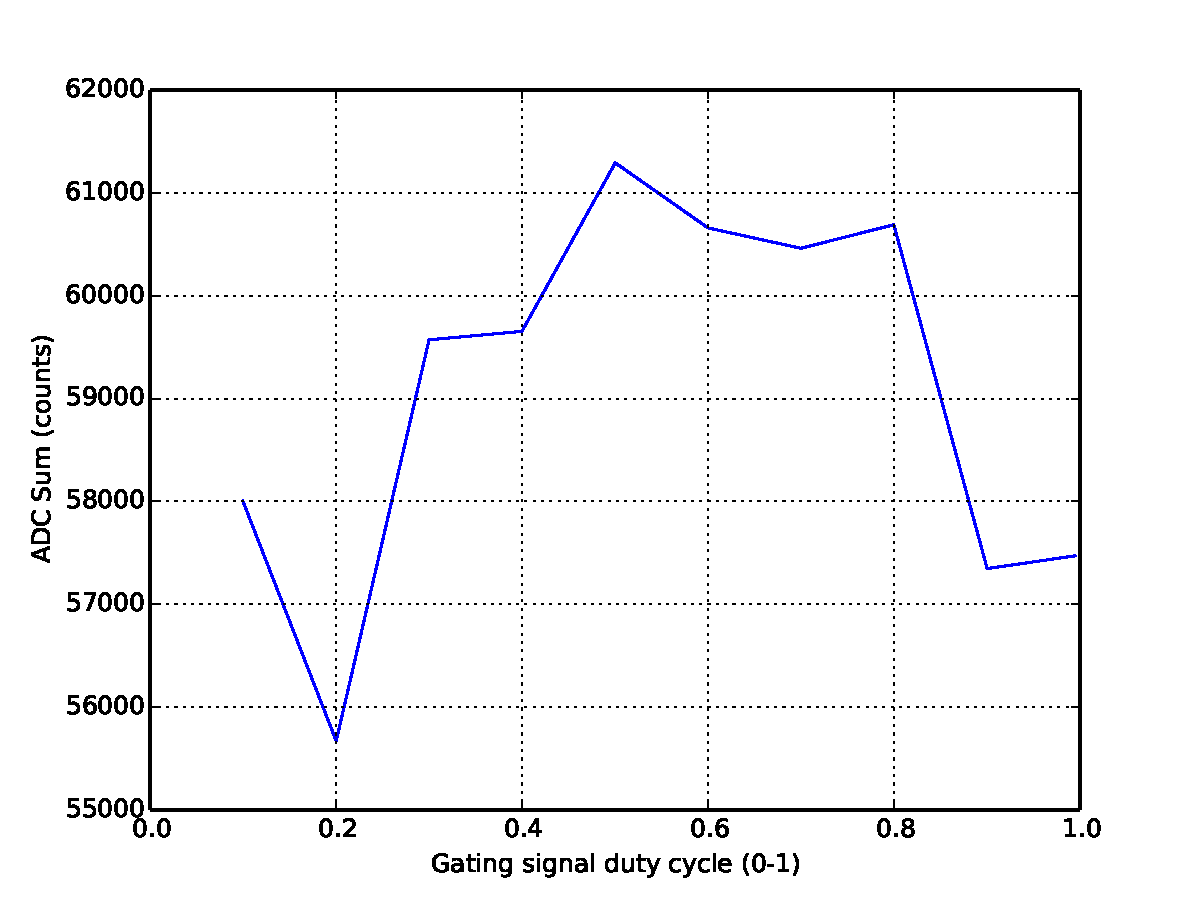
\includegraphics[width=0.8\textwidth]{./Results/scaled_DC_vs_ADC_Sum.pdf}%
\caption{}%
\end{figure}

%
\end{document}